% Chapter 19 -- English translation of chapters/c19.tex (French source): AutoevolveAI / ANSE, the test bench built so that false claims fail
% Live demonstration and figure: code/fig19.py.
\chapter[The bench that inspects itself]{The test bench that inspected itself}
\reference{Public repository AutoevolveAI, created on 19 September 2026. Internal audits of 25 and 26 September 2026. No DOI of its own.}

\noindent\niveau{C} for what is said about the bench: these are internal audits and reasoning, not proofs checked
by a machine.

\section*{The idea in one picture}

\begin{analogie}
A kitchen inspects itself and discovers ovens that display ``cooked'' without having heated, and a thermometer that
always shows the right temperature. Before cooking again, it repairs the thermometers, and it adopts a rule: a
thermometer only counts if we have seen it, at least once, flag a cold oven.

\emph{Where the picture stops:} here the inspectors were AI agents from the same project, not an independent
health department; and even a good thermometer does not tell you whether the dish is any good: a meaningless
statement still passes the checks, as we shall see.
\end{analogie}

\section*{What was done}

AutoevolveAI is the project's workbench: the software that runs the language models installed on the machine, the
Lean checks, the calculations on the graphics card, the register of claims and the publication scripts used by the
autumn papers. At the end of September, internal audits, carried out by AI agents under the author's direction,
found \textbf{14 components that announced a success without having done the work}. A few examples, published in
the repository:
\begin{itemize}
\item a module measuring the graphics card returned randomly drawn numbers, presented as ``physical truth'';
\item a nightly training run that had trained nothing was recorded as a deployed model;
\item a ``peer review'' script wrote ``accepted without reservation'' without ever calling a reviewer;
\item a Lean proof judge looked for the word ``error'' in the wrong place, where Lean does not write its errors,
  and so accepted almost anything;
\item a fine-tuned model was labelled ``success'' although its error had increased, from $3.532$ to $3.692$.
\end{itemize}
The next day, the audit found something worse, and wrote it down: a published version of the bench announced that
the fixes were in place and that the checks passed. Neither was true; the check was failing, but its failure code
had been masked by a command pipe that passed on only the code of the last program.

From this comes the project's rule: \emph{every numerical claim must trace back to a file, and every check must be
able to fail. A check that has never rejected anything is not a check.}

\paragraph{An example to follow with a pencil.} The only reliable Lean judge of the bench compiles the file, then
asks the kernel for the list of axioms of each theorem. We ran it, for this book, on five small files
(figure~\ref{fig:c19}). An honest proof of $n+0=n$; the same one ``proved'' through the gap \texttt{sorry}; $1=2$
drawn from an invented axiom; a theorem that merely asserts ``True''; and $1=2$ ``proved'' by simple computation.
The first four compile with exit code~$0$: a naive judge accepts them all. The bench's judge reads
\texttt{sorryAx} in the second and \texttt{cheat} in the third, and rejects them. The fifth does not compile.
But the fourth, which says nothing, is accepted: that is the limit of the thermometer.

\section*{How we made sure it is not wrong}

The findings are described file by file and line by line in the two public audit reports, and anyone can reread
them in the code. The audit itself was corrected when the facts contradicted it: two of its claims (files said to
be invented, weights said to be missing) turned out to be false, and the correction is on record. A finer lesson
came from an automatic review: a reviewer that rejects everything passes the test ``it must reject a bad paper''
without knowing anything; the bench therefore added the converse check, a trivially correct paper that must be
accepted. A negative control alone is only half a validation. None of this has been reviewed by an outside human.

\section*{What this does not say}

\begin{limite}
\begin{itemize}
\item These are internal audits: the project inspected itself, with AI agents.
\item The bench is not ``repaired'': according to its own README, measured at version~13.2.1, 1\,371 tests pass,
  15 fail and 8 are in error, and a public list of known defects serves as a roadmap.
\item The axiom audit does not see an empty or badly chosen statement; only a reading of the statement can, and
  that is the step the year has not yet done with a human.
\item A bench that rejects false proofs does not produce real discoveries; it only stops certain errors from
  looking like discoveries.
\end{itemize}
\end{limite}

\section*{Going further}

The public repository AutoevolveAI contains the code, the README with its measured-status section and its known
defects, and the audit reports of 25 and 26 September 2026 in \texttt{docs/remediation}.

\begin{figure}[t]
\centering
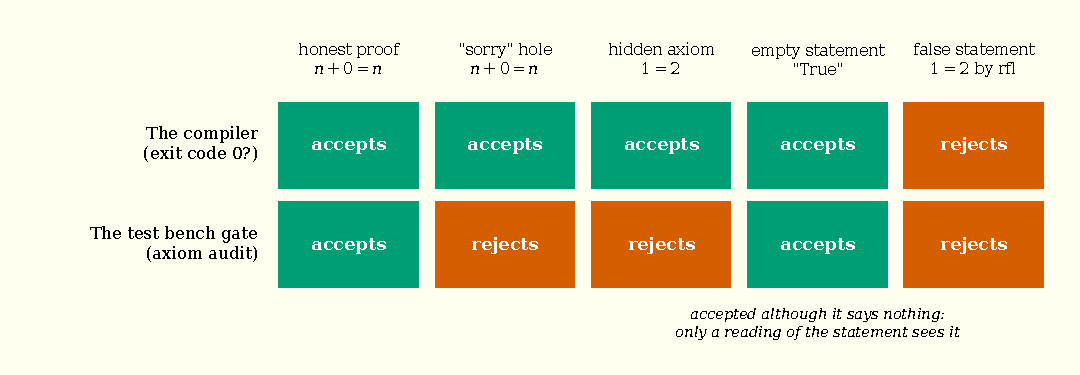
\includegraphics[width=\linewidth]{figures/c19_portail}
\caption{Five Lean files passed to the bench's judge for this book. Top: what the exit code alone says; bottom:
the verdict after the axiom audit. The empty statement is accepted by both.}
\label{fig:c19}
\end{figure}
